\section{Theoretical Analysis}
\label{sec:analysis}
In this section, the circuit shown in Figure~\ref{fig:circuit} is analysed theoretically.
It is important to notice that the purpose is to build a band pass filter circuit using an OPAMP.
This way, the considered circuit has a high pass filter, a signal amplifier (OPAMP) and a low pass filter in series,
where the capacitor C1 and the resistor R1 act as a high pass filter, while capacitor C2 and resistor R2 function as a low pass filter.

Thus, We will begin by computing the gain, input and output impedances at the central frequency.
Then, we will compute the frequency response Vo(f)/Vi(f) , using the incremental circuit, 
solving the circuit for a frequency vector in log scale with 10 points per decade, from 10Hz to 100MHz.
%It is important to notice that, in this analysis, the OP-AMP used is considered ideal, wich means that

%--------------------------------------------------------------------------------------------
\subsection{Gain, Input and Output Impedances at central frequency}
In this subsection, we will compute the gain, input and output impedances at the central frequency.

First, we will calculate low and high cutoff frequencies, $w_L$ and $ w_H$, respectively, as well as central frequency, $w_O$, which are given by:
\begin{equation}
	w_L=\frac{1}{R_{1} \cdot C_{1}}
\end{equation}
\begin{equation}
	w_H=\frac{1}{R_{2} \cdot C_{2}}
\end{equation}
\begin{equation}
	w_O=\frac{1}{ \sqrt{w_{L} \cdot w_{H}}}
\end{equation}

Their values are presented in the table below:
\begin{table}[H]
  \centering
  \begin{tabular}{|l|r|}
     \hline    
    {\bf Name} & {\bf Value} \\ \hline   
    $w_{L}$ & 5.000000e+03 rad/s \\ \hline
$w_{H}$ & 9.090909e+03 rad/s \\ \hline
$w_{O}$ & 6.741999e+03 rad/s \\ \hline
$f_{O}$ & 1.073022e+03 Hz \\ \hline

  \end{tabular}
  \caption{Frequencies}
  \label{tab:freq}
\end{table}

Now we can determine the gain at central frequency, wich is given by the following equation:
\begin{equation}
	T_{w_O}=\frac{R_1\cdot C_1 \cdot jw_O}{1+R_1*C_1*jw_O}\cdot(1+ \frac{R_3}{R_4}) \cdot \frac{1}{1+R_2 \cdot C_2\cdot jw_O}
\end{equation}
, where $R_4$ is the $R_{4a}$ and $R_{4b}$ equivalent resistor.

As well as $Z_{in}$ and $Z_{out}$, at the central frequency, are determined by:
\begin{equation}
	Z_{in}=\frac{R_1\cdot C_1 \cdot jw_O}{1+R_1*C_1*jw_O}\cdot(1+ \frac{R_3}{R_4}) \cdot \frac{1}{1+R_2 \cdot C_2\cdot jw_O}
\end{equation}
\begin{equation}
	Z_{out}=R_1+\frac{1}{jw_O*C_1}
\end{equation}

The results are shown in table~\ref{tab:results1}:
\begin{table}[H]
  \centering
  \begin{tabular}{|l|r|}
     \hline    
    {\bf Name} & {\bf Value} \\ \hline   
    $Z_{in}$ & 9.090909e+02 + j-6.741999e+02 Ohm \\ \hline
$Z_{out}$ & 6.451613e+02 + j-4.784644e+02Ohm \\ \hline
$|Z_{in}|$ & 1.131809e+03 Ohm \\ \hline
$|Z_{out}|$ & 8.032193e+02 Ohm \\ \hline

  \end{tabular}
  \caption{Results at central frequency}
  \label{tab:results1}
\end{table}

\subsection{Frequency response Vo(f)/Vi(f)}
Now, considering the transfer function $T(s)$, it is given by:
\begin{equation}
	T(s)=\frac{V_out(s)}{V_in(s)}=1+\frac{Z_{in}(s)}{Z_{out}(s)}=\frac{R_1\cdot C_1 \cdot s}{1+R_1*C_1*s}\cdot(1+ \frac{R_3}{R_4}) \cdot \frac{1}{1+R_2 \cdot C_2\cdot s}
\end{equation}
, where $\frac{R_1\cdot C_1 \cdot s}{1+R_1*C_1*s}$, $1+\frac{R_3}{R_4}$ and $\frac{1}{1+R_2\cdot C_2\cdot s}$ represent
the gain at high pass filter, OP-AMP and low pass filter, respectively.

This way, the gain frequency response is plotted in the figure below.
\begin{figure}[H] \centering
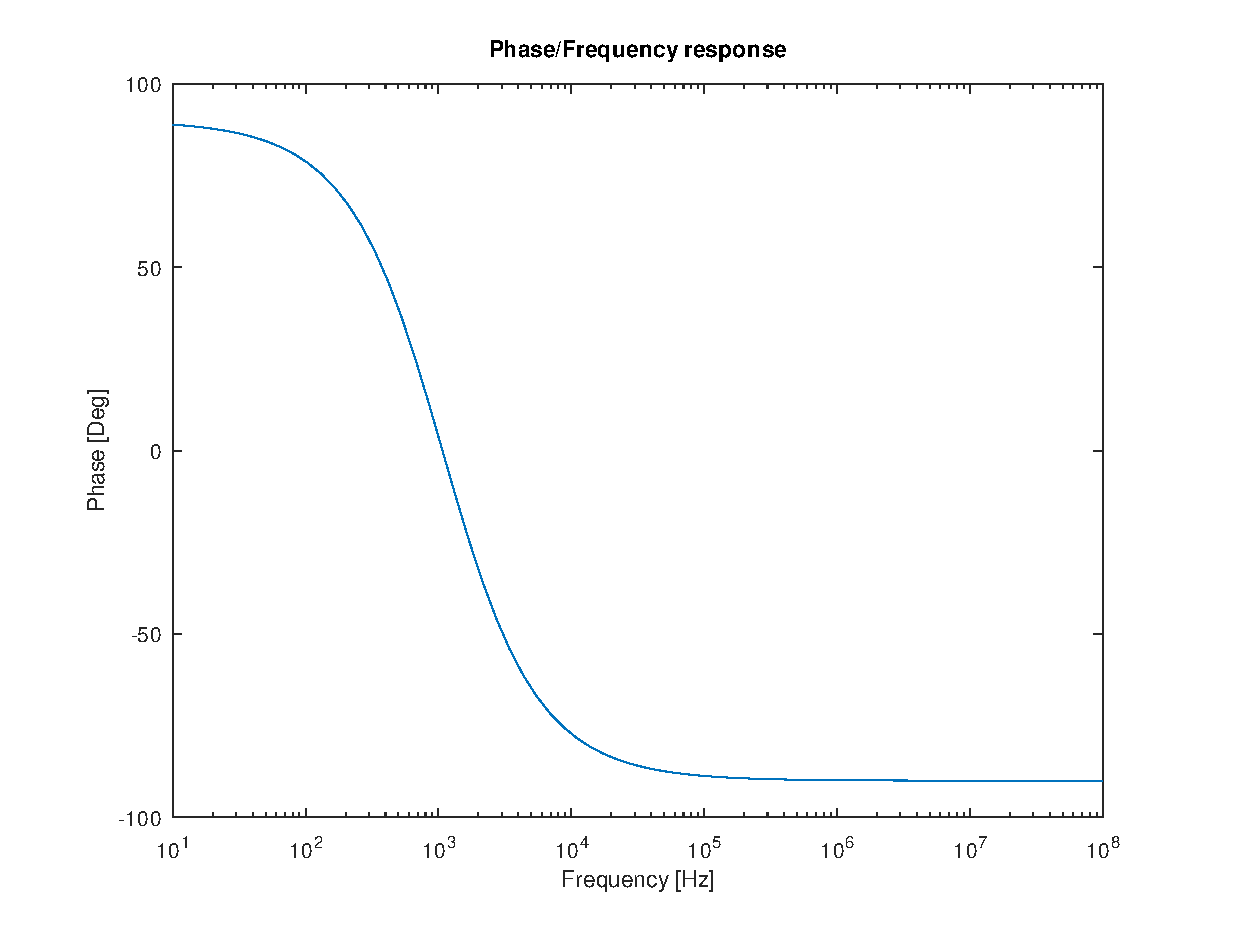
\includegraphics[width=0.6\linewidth]{phase_response.eps}
\caption{Phase Frequency Response}                         %%%%%%%%%%LEGENDA
\label{fig:phasef}
\end{figure}
\begin{figure}[H] \centering
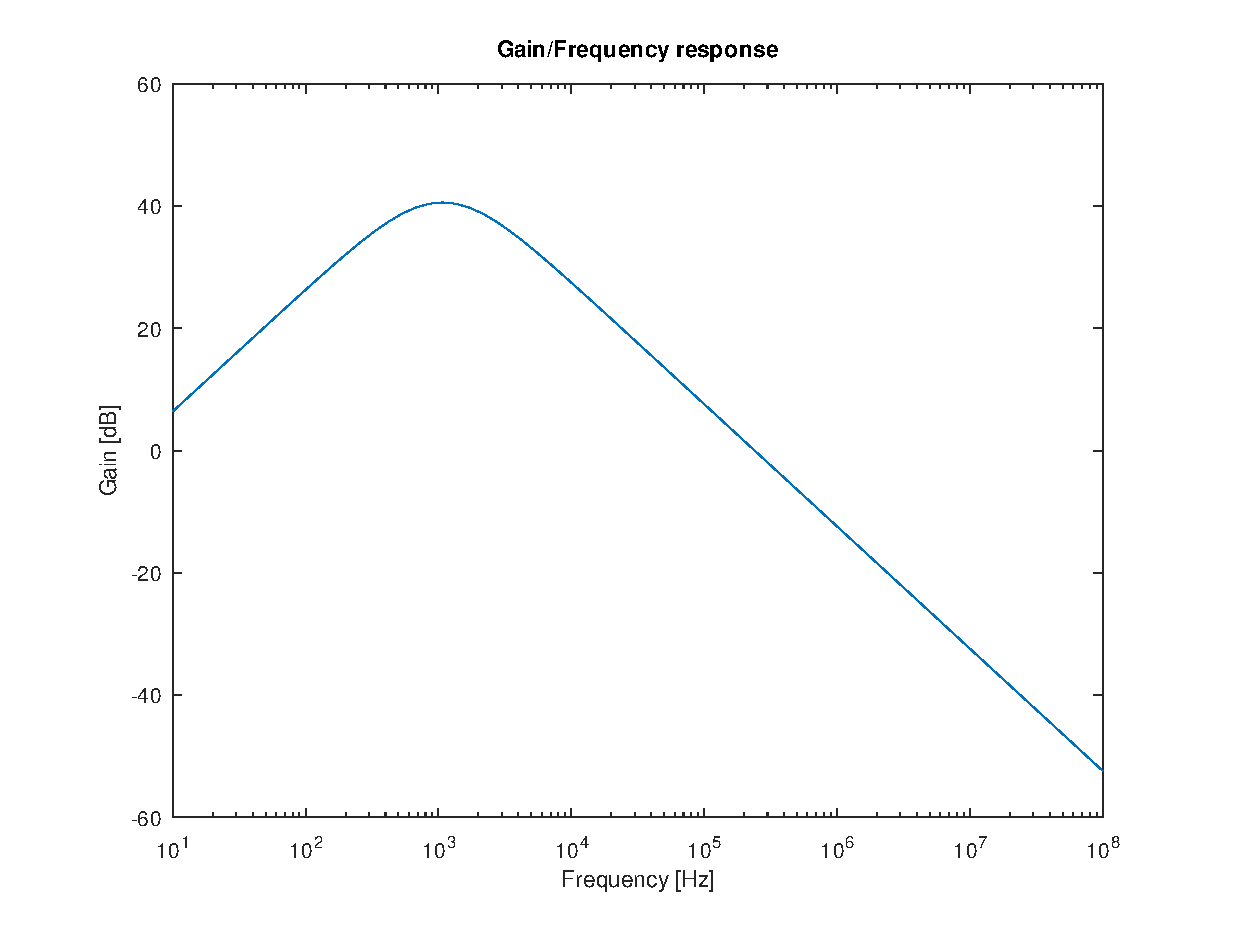
\includegraphics[width=0.6\linewidth]{gain_response.eps}
\caption{Gain Frequency Response}                         %%%%%%%%%%LEGENDA
\label{fig:gainf}
\end{figure}
As we can see there is a maximum for the frequencies in the central frequency, wich is near to 1KHz, otherwise low and high frequencies have a low gain. That was expected because
both low and high frequencies were blocked by high and low pass filters.

%\subsection{Comparison}

%Table~\ref{tab10:sim} presents the simulation results for the circuit under analysis.

%\begin{table}[H]
%  \centering
%  \begin{tabular}{|l|r|}
%    \hline    
%    {\bf Name} & {\bf V or dB} \\ \hline
%    \input{../sim/sim_tab}
%  \end{tabular}
%  \begin{tabular}{|l|c|}
%    \hline
%    {\bf Impedance} & {\bf kOhms} \\ \hline
%    zin & 2.236262e+00\\ \hline

%  \end{tabular}
%  \begin{tabular}{|l|c|}
%    \hline
%    {\bf Impedance} & {\bf kOhms} \\ \hline
%    \input{../sim/output_tab2}
%  \end{tabular}
%    \caption{Simulation Results.}
%    \label{tab10:sim}
%\end{table}

%Comparing with the theoretical ones, we can see that they are slightly different, result of the fact that the theoretical model is an approximation and the transistors used in NGSpice were real. However, the results obtained are satisfatory!
